\documentclass[12pt]{article}
\usepackage[utf8]{inputenc}
\usepackage{graphicx}
\usepackage[a4paper,width=150mm,top=25mm,bottom=25mm]{geometry}

\title{

\\
{COS 301 SRS}
}



\author{Ctrl Alt Defeat}

\begin{document}

\begin{titlepage}
    \centering



    \vspace{2cm}
    \hrulefill\\
    \vspace{1cm}
    {\Huge\bfseries SRS Documentation v3.0}

    \vspace{1cm}

    {\Large Software Requirements Specification Document for\\Domain Pulse}\\
    \vspace{1cm}
    \hrulefill\\

    \vfill

    {\large Ctrl Alt Defeat}

    \vspace{1cm}

    {\large 2023/07/31}\\
    %    \vspace{1cm}
    %    \vspace{1cm}
    %    
\includegraphics[width=10cm]{../../Images/dpLogo.png}
    %    \vspace{1cm}\\
    %    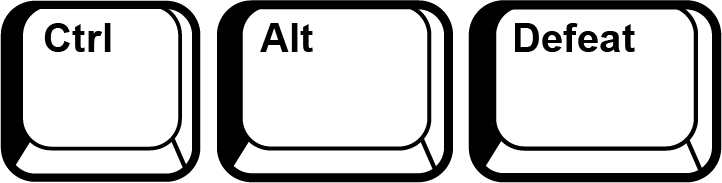
\includegraphics[width=6cm]{../../Images/cadLogo.png}

\end{titlepage}



\tableofcontents

\newpage











\section{Introduction}

\subsection{Overview}
Introducing Domain Pulse, the ultimate sentiment analysis platform. With Domain Pulse, you can easily gauge the sentiment surrounding any domain. Whether it's a business, a person, or anything else, Domain Pulse gathers information from across the internet and analyzes what people are saying.\\
\\Domain Pulse presents the results in a visually stunning and easy-to-understand format. Our wide range of visualizations brings statistics to life, making it a breeze to grasp the online presence and sentiment for any domain. Take control of understanding public opinion like never before with Domain Pulse.
\subsection{Objectives}

The objectives of the Domain Pulse project are to develop a comprehensive web application that enables users to track and analyze data from multiple sources, perform sentiment analysis, and visualize statistics. The application aims to provide a user-centered design approach, ensuring usability, accessibility, and a clear and intuitive interface. The system will be built using a scalable and modifiable architecture, leveraging microservices to handle high traffic and enable easy modification and extension. Security will be a top priority, with encryption and access control measures in place to protect user data. The project also aims to achieve high performance through caching and database optimization techniques. Overall, the objective is to create a reliable and efficient platform that empowers users to gain valuable insights from data analysis.

\newpage













\section{User Characteristics}

\subsection{Demographics}
\begin{itemize}
  \item \textbf{Age}: Users of varying age groups, depending on their professional roles and interests.
  \item \textbf{Gender}: Users of all genders.
  \item \textbf{Education Level}: Users with diverse educational backgrounds.
  \item \textbf{Occupation}: Business professionals, social media managers, researchers, PR professionals, etc.
\end{itemize}

\subsection{Psychographics}
\begin{itemize}
  \item \textbf{Attitudes}: Users interested in sentiment analysis, monitoring online presence, and understanding public perception.
  \item \textbf{Values}: Users who value data-driven decision-making and insights for decision support.
  \item \textbf{Interests}: Users interested in market research, branding, reputation management, and online sentiment analysis.
  \item \textbf{Lifestyles}: Users with professional roles that involve monitoring and managing online presence and sentiment.
  \item \textbf{Personality Traits}: Users with analytical and research-oriented mindsets.
\end{itemize}

\subsection{Technological Proficiency}
\begin{itemize}
  \item \textbf{Novice Users}: Users with basic technological skills who may require more guidance.
  \item \textbf{Intermediate Users}: Users with moderate experience and comfort using technology.
  \item \textbf{Expert Users}: Users who are technologically proficient and can quickly adapt to new systems.
\end{itemize}

\subsection{Physical Abilities}
\begin{itemize}
  \item \textbf{Vision}: Users with varying visual abilities.
  \item \textbf{Other Physical Abilities}: Consideration for accessibility and usability for all users.
\end{itemize}

\subsection{Cognitive Abilities}
\begin{itemize}
  \item \textbf{Attention}: Users with different levels of attention spans.
  \item \textbf{Memory}: Users with varying memory capabilities.
\end{itemize}

\subsection{Prior Knowledge and Experience}
\begin{itemize}
  \item Users with different levels of knowledge and experience in sentiment analysis and online presence monitoring.
  \item Familiarity with Similar Tools or Platforms
\end{itemize}

\subsection{Goals and Tasks}
\begin{itemize}
  \item Monitoring and analyzing sentiment and online presence of specific domains.
  \item Gathering insights for decision-making, market research, or branding purposes.
  \item Tracking public perception, PR campaign impact, or personal brand sentiment.
  \item Supporting research and analysis with data on sentiment trends and patterns.
\end{itemize}

\subsection{Emotional Factors}
\begin{itemize}
  \item Users with preferences for user interfaces and interactions that evoke positive emotions.
  \item Designing a user experience that is intuitive, engaging, and delightful.
\end{itemize}

\newpage
















\section{User Stories}

\newpage

\section{Functional Requirements}

\subsection{Requirements}

\subsection{Use Case Diagrams}
\begin{center}
    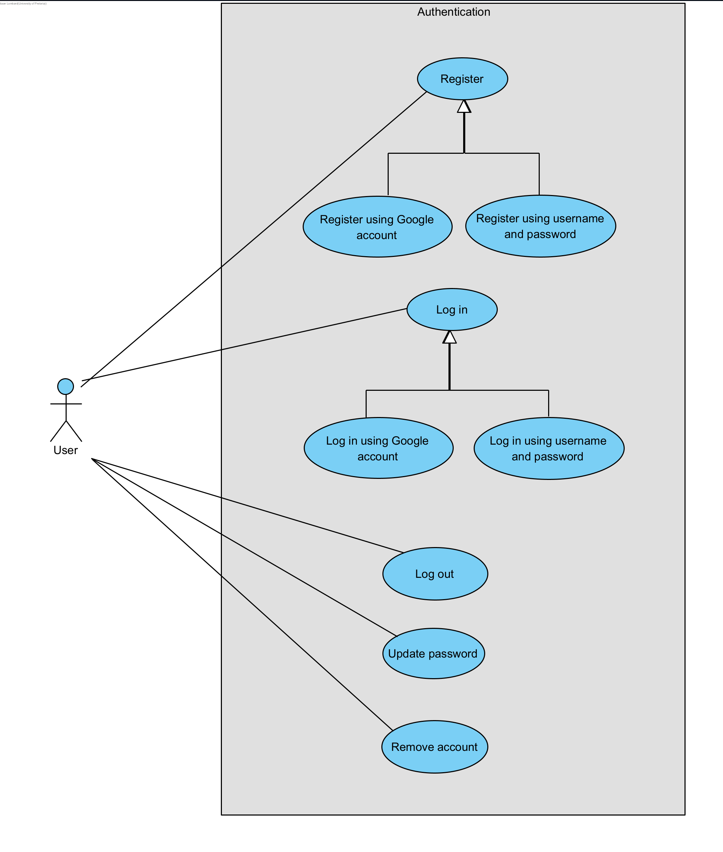
\includegraphics[width=13cm]{../../Images/uc1.1.png}
    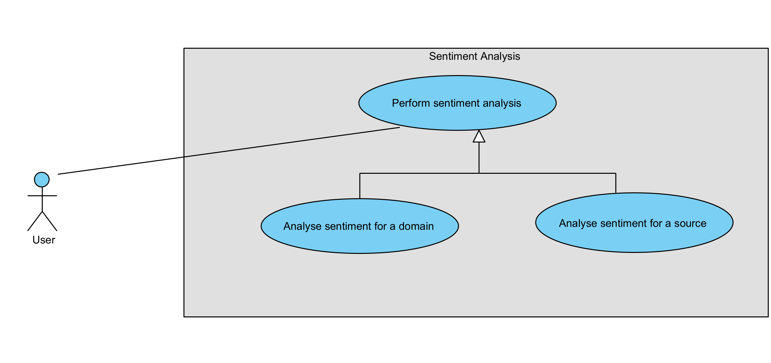
\includegraphics[width=13cm]{../../Images/uc1.2.png}
    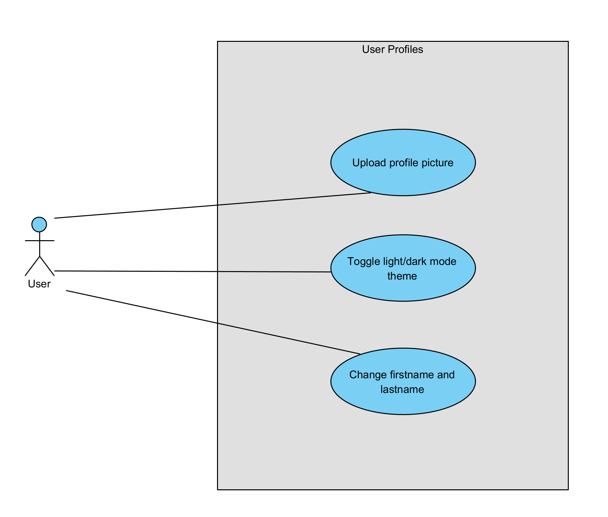
\includegraphics[width=13cm]{../../Images/uc1.3.png}
    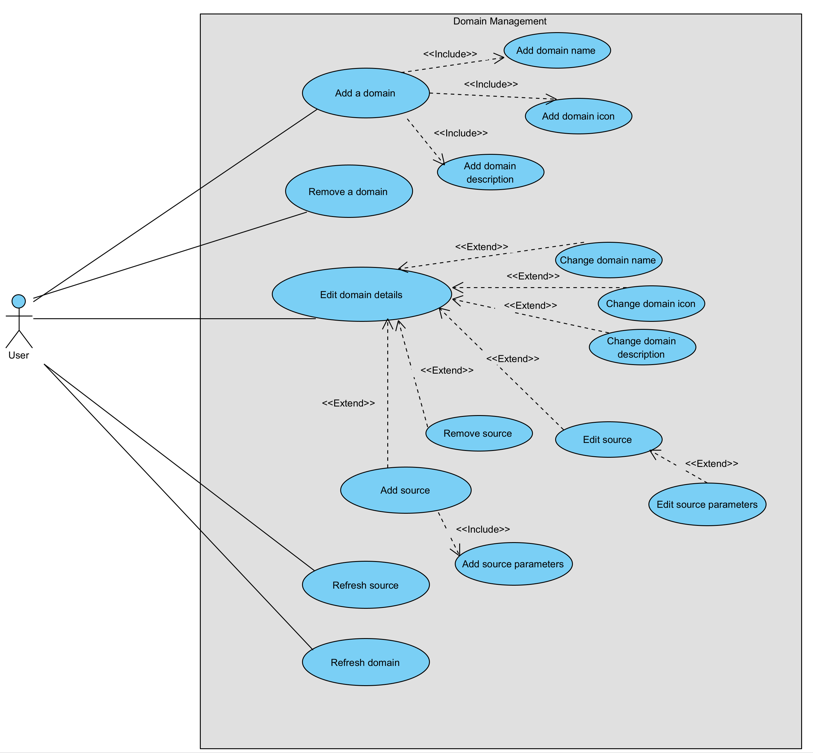
\includegraphics[width=13cm]{../../Images/uc1.4.png}
    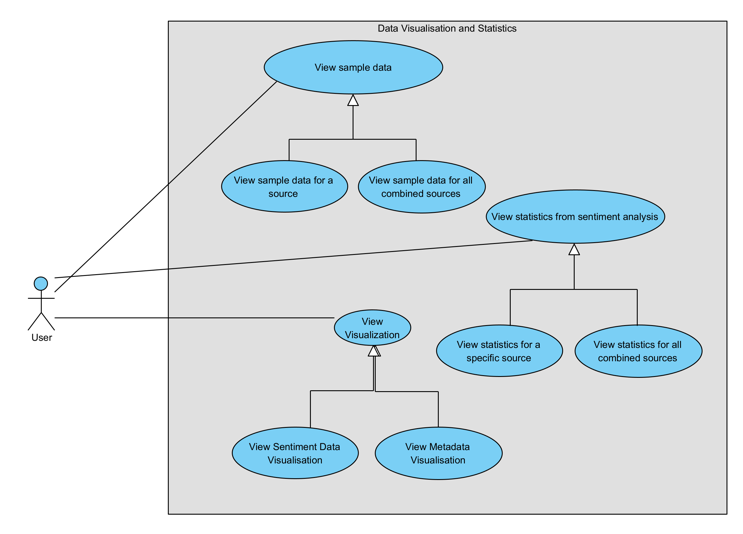
\includegraphics[width=13cm]{../../Images/uc1.5.png}
\end{center}




\newpage

\section{Service Contract}

\newpage

\section{Contract Design}

\newpage

\section{Database Design}

\newpage

\section{Class Diagram}

\newpage

\section{Architectural Requirements}

\subsection{Quality Requirements}

\begin{itemize}
    \item Security
    \item Usability
    \item Accessibility
    \item Scalability
    \item Availability
    \item Modifiability
    \item Performance
  \end{itemize}

\subsection{Architectural Patterns and Tactics}

Below we discuss which architectural patterns and tactics we will use to meet the quality requirements. The patterns and tactics are in bold.

\subsubsection*{Security}

\subsubsection*{Usability}

\begin{itemize}
    \item User-Centred Design Approach
    \begin{itemize}
    \item Consider the end-user throughout the design process and design the system accordingly.
    \item Make the terminology easy to understand but still meaningful, considering users with no technical knowledge about NLP (Natural Language Processing).
    \item Examples of end-users: R\&D specialists, social media managers, project leaders, executives, consultants.
    \end{itemize}
    \item Clear and Intuitive Interface
    \begin{itemize}
    \item Reduce clutter on the dashboard.
    \item Ensure that the meaning and purpose of actions is clear through the use of descriptive and minimalistic icons.
    \item Provide user feedback as they navigate through the application.
    \item Utilize a user workflow of top-to-bottom, left-to-right navigation, ensuring that the process of completing steps feels natural and ordered.
    \end{itemize}
    \item Usability Testing
    \begin{itemize}
    \item Test the system with representative users.
    \item Collect and implement feedback.
    \end{itemize}
\end{itemize}

\subsubsection*{Accessibility}

\begin{itemize}
    \item Implement a Dark Mode
    \begin{itemize}
    \item Cater to visually impaired and cognitive disabilities by providing a simple, distraction-free, high contrast user interface.
    \end{itemize}
\end{itemize}

\subsubsection*{Scalability}

\subsubsection*{Availability}

\subsubsection*{Modifiability}

\subsubsection*{Performance}

  


\newpage

\section{Quality Requirements}

\newpage

\section{Architectural Patterns and Tactics}

\newpage

\section{Design Patterns}

\newpage

\section{Constraints}

\newpage

\section{Technology Requirements}

\newpage



\end{document}
